\chapter{Experimental results}
\label{cpt:experiments}

\begin{table}[h]
	\centering
	\begin{tabular}{l|l}
		\textbf{Component} 	& \textbf{Specifications} \\ \hline
		OS   				& Ubuntu 15.10 \\
		Python version		& 2.7.10 \\
		CPU					& 1 Core with 4 processors (2.5 GHz each) \\ 
		HDD					& 25 GB  \\ 
		RAM					& 8 GB  \\
	\end{tabular}
	\caption{Specifications of the setup used during the idle iotop measurement of Tribler 6.6.0-pre-exp.}
	\label{table:virtual_machine_specs}
\end{table}

To evaluate Tribler's current situation and to validate our implementations are working correctly, experiments have been conducted.
In this chapter we elaborate on these experiments and discuss the results. 
All experiments with the exception of one have been conduction on a virtual private server whose specifications can be found in Table\ref{table:virtual_machine_specs}.

\section{Tribler's I/O over the years}
As explained earlier, Tribler's I/O has been a problem for years.
To observe if and how the amount of I/O has changed over time, we have performed measurements on four \todo{change if needed} different versions of Tribler using iotop\footnote{\url{http://guichaz.free.fr/iotop/}}.
The versions and their release dates are depicted in Table~\ref{table:tribler_version_dates}.

As these measurements were never performed systematically, it is vital to perform these measurement now to observe if any changes have occurred between releases and document them.
This will provide valuable insight in Tribler's behaviour and the extent of the problem.
Moreover it will show us if the amount of I/O is being reduced since the creating of the ticker on GitHub.

\begin{table}[h]
	\centering
	\caption{The versions of Tribler and their release dates.}
	\label{table:tribler_version_dates}
	\begin{tabular}{|l|l|}
		\hline
		Tribler version & Release date \\ \hline
		6.3.5           & 2014-11-06   \\ \hline
		6.4.3           & 2015-01-21   \\ \hline
		6.5.2           & 2016-05-13   \\ \hline
		6.6.0-exp1      & 2016-07-26   \\ \hline
	\end{tabular}
\end{table}

\begin{figure}[!h]
	\centering
	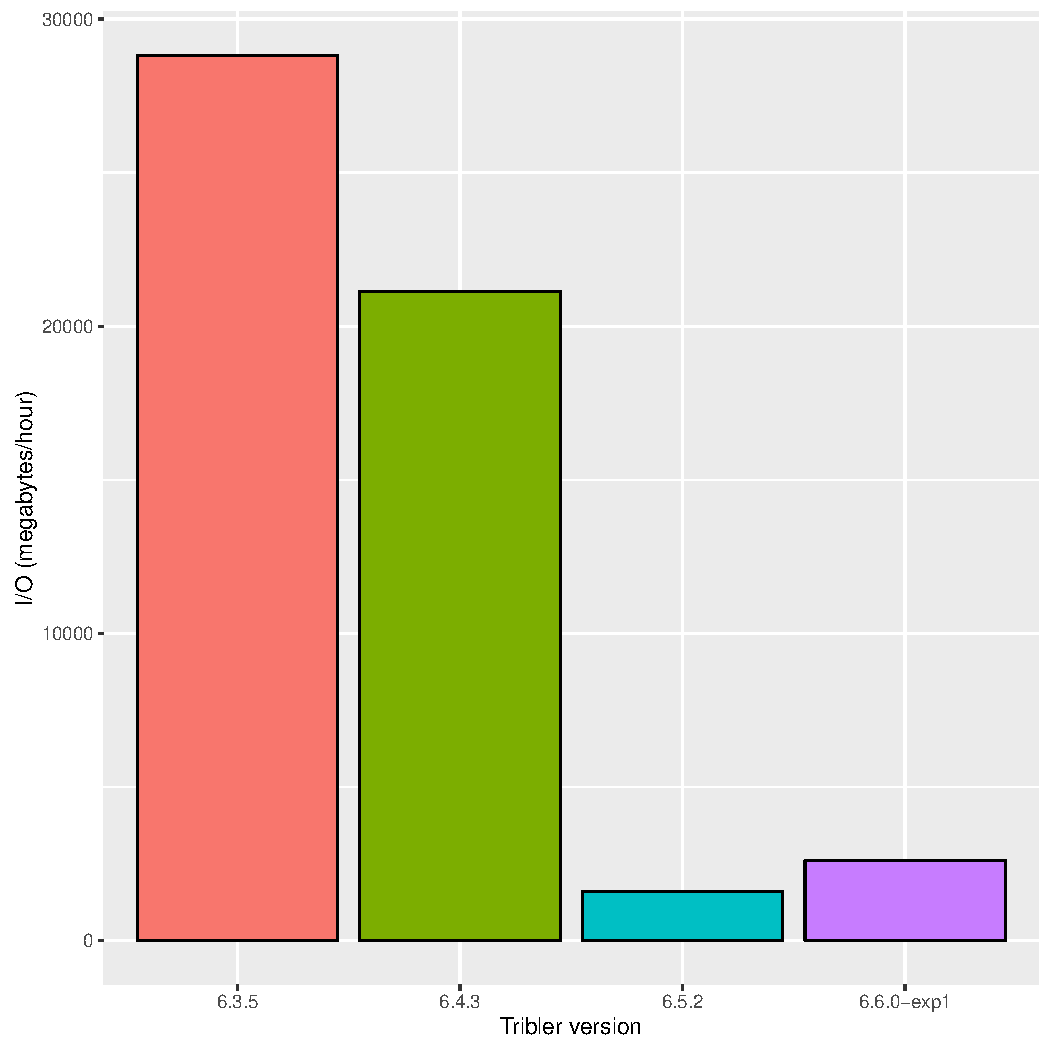
\includegraphics[width=\linewidth]{experimentation/images/io_history}
	\caption{The amount of I/O per version of Tribler.}
	\label{fig:io_history}
\end{figure} 

Each version of Tribler will run for one hour idle, using a clean state directory i.e. no prior knowledge of the network and its contents.
During the idle run, Tribler will start discovering peers and content such as channels and torrents, storing the obtained data in the database which gets flushed to disk.
Additionally, peers will start requesting data from this Tribler instance such as search and peer exchange requests, causing Tribler to read data from the database.
These read and writes operations will be monitored by iotop and the amounts automatically accumulated.
After one hour, the amount of read and write I/O is noted down and Tribler is shutdown.

The results of this experiment are visible in Figure~\ref{fig:io_history}.
From this figure we observe that Tribler's I/O has reduced significantly in version 6.5.2, yet is climbing again in the latest release due to the MultiChain feature added. 

Additionally, the numbers observed in this experiment are significantly higher than the numbers reported in the original ticket.
We believe the reason for this is due to the 100 mbit connection of the experiment machine, providing excellent connectability conditions. 
Secondly, the fact that it began with a clean state directory while running idle, provides ideal conditions for Tribler to spend most of its resources on discovering peers and content.

Finally, we observe that the total amount of I/O the latest version of Tribler is performing is 2598 MB/hour.
This shows the urgency of the I/O to become asynchronous and non-blocking.

\section{I/O breakdown}

\begin{table}[]
	\centering
	\caption{A breakdown of the functions called on StormDBManager.}
	\label{table:breakdown_tribler_idle}
	\begin{tabular}{|l|r|r|l|l|l|}
		\hline
		\textbf{Query}	& \textbf{Amount of calls} & \textbf{Total time (s)} & \textbf{Max}  & \textbf{Average} & \textbf{Min} \\ \hline
		fetchone	& 83036	& 3361.644 	& 0.81436	& 0.04048	& 0.00006 \\ \hline
		fetchall	& 2569	& 22.512	& 0.66344	& 0.00876	& 0.00007 \\ \hline
		execute		& 422	& 2.326  	& 0.20488	& 0.00551	& 0.00007 \\ \hline
		executemany	& 1		& 0.009 	& 0.00915 	& 0.00915	& 0.00915 \\ \hline
	\end{tabular}
\end{table}

To observe the individual components separately, we have created a breakdown of the database queries performed by Tribler and Dispersy.
We have run Tribler idle for one hour and tracked how many times each function in StormDBManager was called by either Dispersy or Tribler and how long it takes between scheduling the query the callback being invoked.
A breakdown of the functions is visible in Table~\ref{table:breakdown_tribler_idle}.
From this table we see that the \enquote{fetchone} function is being called the most, but what does this mean\todo{change and elaborate}

\section{Tribler's performance}

To measure the performance gain of Tribler, we have conducted two sets of experiments where two instances of Tribler, one with a synchronous, blocking Dispersy implementation and one with the asynchronous, non-blocking version of Dispersy, are compared.

In the first experiment we have ran Tribler idle for one hour while querying the Twisted event loop every 100 milliseconds for delayed calls.
By doing so we can observe if certain tasks have been delayed past their set time of execution i.e. measure the latency in the system.

In the second experiment we have stress-tested Tribler's new API.
By requesting data from an endpoint at several rates per second, we can observe the throughput, response times, variance in these response times and throughput of Tribler.

\subsection{Measuring the latency of Tribler}

\begin{table}[h]
	\centering
	\begin{tabular}{l|l}
		\textbf{Component} 	& \textbf{Specifications} \\ \hline
		Operating System   	& Ubuntu 16.04 LTS \\
		Python version		& 2.7.12 \\
		CPU					& Intel Core i5-2410M \\ 
		HDD					& Samsung 850 EVO 250GB  \\ 
		RAM					& 8 GB DDR3 1600MHz \\
	\end{tabular}
	\caption{Specifications of the setup used during the idle iotop measurement of Tribler 6.6.0-pre-exp.}
	\label{table:tribler_idle}
\end{table}

In this experiment we have compared two versions of Tribler, one with Dispersy having  blocking, synchronous I/O and one with Dispersy running StormDBManager and thus having non-blocking, asynchronous I/O.
Each instance of Tribler was run one hour idle where every 100 milliseconds the event loop of Twisted was queried for delayed calls.
By observing if scheduled calls are past their set time of execution, we can measure the amount of delay or \emph{latency} in the system.
Latency occurs when the twisted reactor thread is blocked or busy with a task that takes a relative long time to complete, causing other tasks to become delayed.
Latency is therefore directly related to the responsiveness of a program.
The lower the latency, the more responsive a system is.

In theory, making functions asynchronous slices them into smaller \enquote{chunks} which can be executed interleaved, creating a more responsive system as e.g. user actions will be executed in between (background) operations.

In this experiment the hypothesis is that the latency of the asynchronous version will be lower than its synchronous counterpart.
Since Tribler is running idle it has more resources i.e. CPU time available to tend to Dispersy which is running in the background, which most likely will cause the difference to be smaller than when Tribler is experiencing additional load.
However, we believe the average may still be significant enough to prefer the asynchronous implementation.

\begin{figure}[!h]
	\centering
	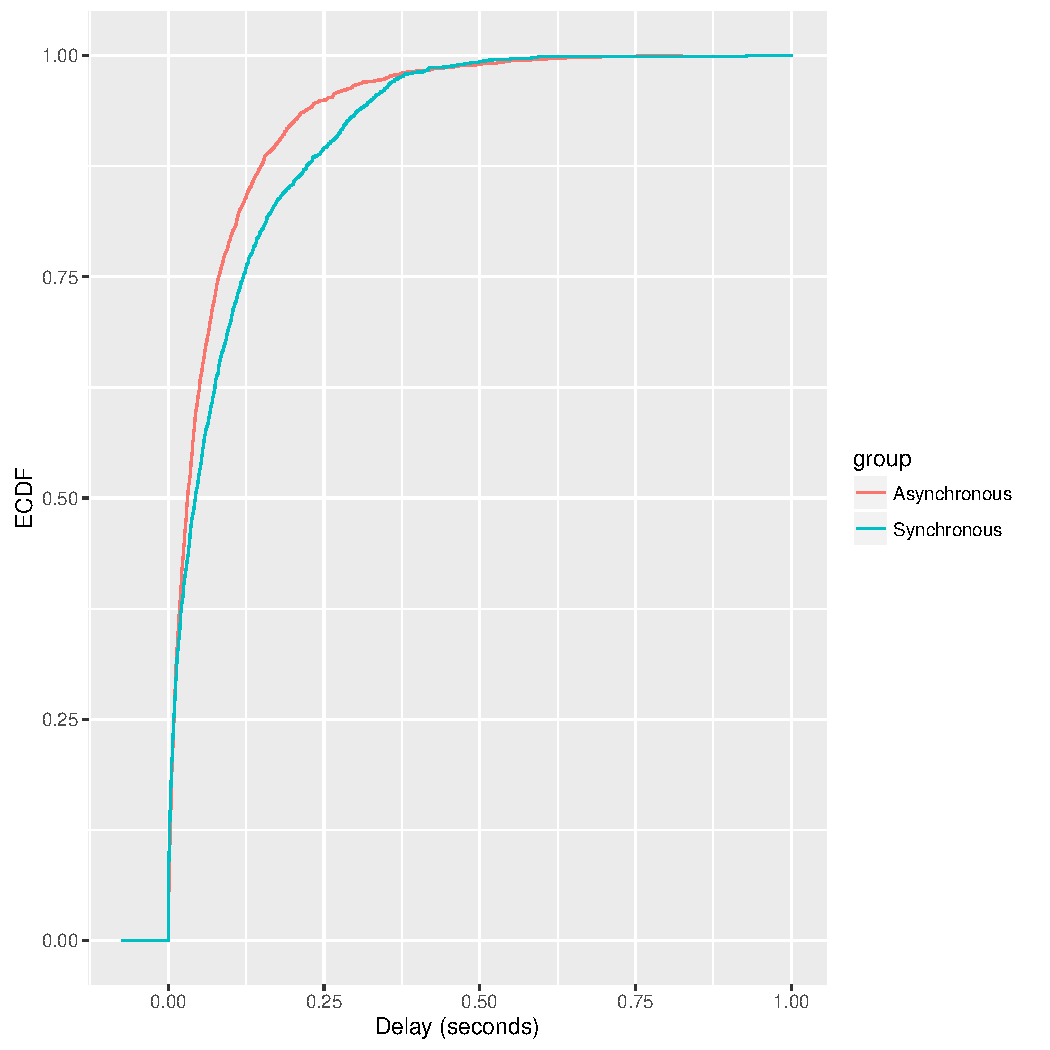
\includegraphics[width=\linewidth]{experimentation/images/ecdf_latency_idle}
	\caption{An ECDF plot of the latency when running Tribler idle.}
	\label{fig:ecdf_latency_idle}
\end{figure} 

After running the experiment, we have created an empirical cumulative distribution function (ECDF) plot of the delayed calls, visible in Figure~\ref{fig:ecdf_latency_idle}.
From this figure we observe that the asynchronous version performs better than the synchronous version.
On average, the synchronous version has a latency of 87 milliseconds, where the asynchronous version has a latency of 66 milliseconds, a difference of 24\%.
Also, the synchronous case has more outliers, some even crossing the one second mark.
This performance gain is significant enough to confirm the hypothesis.

\subsection{Measuring the responsiveness of Tribler}

To measure the responsiveness of Tribler while under load, we have stress tested the API of Tribler.
This API was introduced to run Tribler headless, i.e. without an interface as part of a next major refactoring.
To stress test the Tribler, we have used Apache JMeter\footnote{\url{http://jmeter.apache.org/}}.
Apache JMeter was designed to "simulate a heavy load on a server, group of servers, network or object to test its strength or to analyze overall performance under different load types." (jmeter.apache.org, 2016).

In this experiment we use a state directory containing roughly 1200 channels.
By querying Tribler's channel API endpoint for all discovered channels, all channels in the database will be fetched and returned.
As this is Tribler's heaviest endpoint in terms of computation, it's the best way to put Tribler under load.
In total the experiment will be run six times, every run the channel endpoint will be queried exactly 1000 times, using 1, 2, 5, 10, 15 and 20 requests per second respectively.
By tracking the response times, the amount of requests per seconds and the throughput the API can offer, we can measure the gain in responsiveness and thus in performance of Tribler.
We expect that the asynchronous version will outperform the synchronous version significantly in both response times as throughput.

\begin{table}[!h]
	\centering
	\caption{The results of the six experiments runs with and without asynchronous, non-blocking I/O in Dispersy.}
	\label{table:responsiveness_tribler_load}
	\begin{tabular}{|c|c|c|c|c|c|c|c|}
		\hline
		Req./s              & Async. & avg & min & max  & Std. Dev. & Throughput (KB/s) & responses/s \\ \hline
		\multirow{2}{*}{1}  & \xmark      & 315 & 53  & 4774 & 615.90    & 564.19            & 0.9         \\ \cline{2-8} 
		& \cmark      & 134 & 57  & 2576 & 189.89    & 612.60            & 1.0         \\ \hline
		\multirow{2}{*}{2}  & \xmark       & 237 & 52  & 4524 & 475.31    & 1049.31           & 1.7         \\ \cline{2-8} 
		& \cmark      & 113 & 56  & 1224 & 162.62    & 1197.90           & 1.9         \\ \hline
		\multirow{2}{*}{5}  & \xmark       & 143 & 52  & 2865 & 259.64    & 2399.57           & 3.9         \\ \cline{2-8} 
		& \cmark      & 67  & 56  & 846  & 38.50     & 3058.27           & 5.0         \\ \hline
		\multirow{2}{*}{10} & \xmark       & 135 & 54  & 3338 & 259.37    & 3827.02           & 6.2         \\ \cline{2-8} 
		& \cmark      & 89  & 52  & 1138 & 92.58     & 5435.71           & 8.8         \\ \hline
		\multirow{2}{*}{15} & \xmark       & 133 & 51  & 4678 & 382.57    & 4521.46           & 7.3         \\ \cline{2-8} 
		& \cmark      & 88  & 52  & 963  & 82.23     & 6799.35           & 11.0        \\ \hline
		\multirow{2}{*}{20} & \xmark       & 109 & 51  & 3400 & 239.23    & 5599.75           & 9.1         \\ \cline{2-8} 
		& \cmark      & 74  & 52  & 1051 & 57.37     & 8264.01           & 13.4        \\ \hline
	\end{tabular}
\end{table}

\begin{figure}[!h]
	\centering
	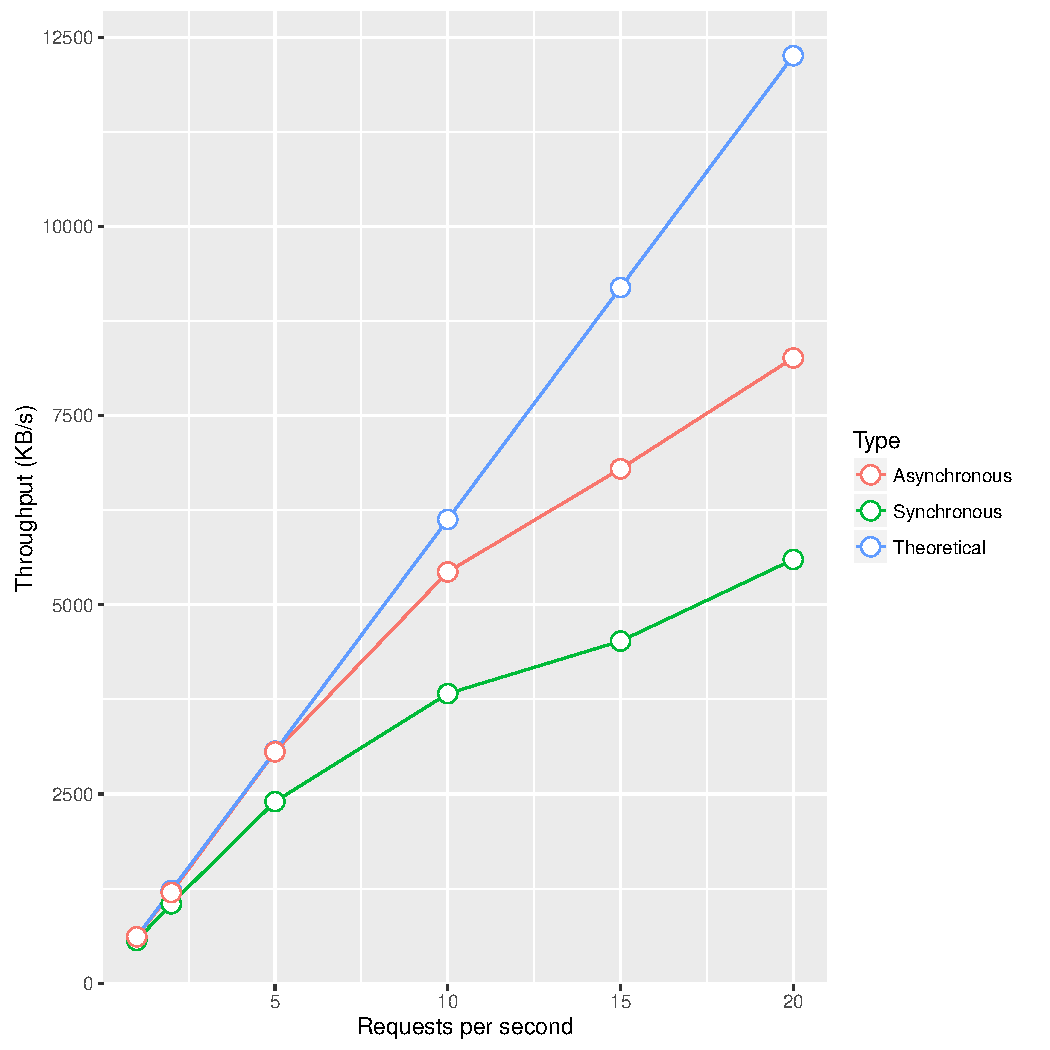
\includegraphics[width=\linewidth]{experimentation/images/throughput_requests.pdf}
	\caption{The throughput theoretically and of Tribler running Dispersy with asynchronous, non-blocking and synchronous, blocking I/O }
	\label{fig:throughput_requests}
\end{figure} 

The results of the experiment can be found in Table~\ref{table:responsiveness_tribler_load}.
From this table we observe that asynchronous version has a significant less amount of response time, both on average and in maximal duration.
The reduction in response times (on average) ranges between 32.1\% and 57.5\%.
The standard deviation is also significantly less, indicating the response times are more stable than the synchronous version.
Yet perhaps the most promising statistic is the throughput.
As the response is 613 kilobytes (KB) in size, the theoretical maximum throughput will be 613, 1226, 3065, 6130, 9195 and 12260 KB/s, respectively.
If we plot the theoretical, asynchronous and the synchronous throughput we obtain Figure~\ref{fig:throughput_requests}.
As we can see the throughput of the asynchronous case lies close to the theoretical maximum until around the ten requests per second.
At this point Tribler starts to show signs of being overloaded, which is also visible in the Table~\ref{table:responsiveness_tribler_load} when looking at the amount of responses received per second.
Nonetheless, this demonstrates that the asynchronous system has superior performance over the synchronous case, increasing the throughput up to 150\%.

\todo{Maybe plot the response times over time? per request Async should be more smooth. I could also create a comparison graph and show this in the performance regression chapter?}

\section{Scalability}

If allchannel works, talk about scalability of nodes. \todo{todo}


